% !TEX encoding = UTF-8
% !TEX program = pdflatex
% !TEX root = MEMOC.tex
% !TEX spellcheck = it-IT
\documentclass[a4paper, 11pt]{report} % Font size (can be 10pt, 11pt or 12pt) and paper size (remove a4paper for US letter paper)
\usepackage[italian]{babel}      							% Lingua italiana
\usepackage[margin=.9in]{geometry}             % Imposta i margini del documento

\usepackage[T1]{fontenc} % Required for accented characters
\usepackage[mathletters]{ucs}    % Caratteri matematici come UTF8
\usepackage[utf8,utf8x]{inputenc}      % Ancora utf8

\usepackage{eurosym}                %simbolo dell'euro
\usepackage{listings}
\usepackage[usenames,dvipsnames,svgnames,table]{xcolor}
% Imposta lo spazio nella list of listing in modo simile alla list of figures/tables
%\makeatletter
%\let\my@chapter\@chapter
%\renewcommand*{\@chapter}{%
%  \addtocontents{lol}{\protect\addvspace{10pt}}%
%  \my@chapter}
%\makeatother


\definecolor{codegreen}{rgb}{0,0.6,0}
\definecolor{codegray}{rgb}{0.5,0.5,0.5}
\definecolor{backcolor}{rgb}{0.98,0.98,0.98}

\renewcommand{\lstlistingname}{Codice}% Listing -> codice
\renewcommand{\lstlistlistingname}{Elenco dei frammenti di codice}% List of Listings -> Frammenti di codice

\lstdefinestyle{mystyle}{
    backgroundcolor=\color{backcolor},   
    commentstyle=\color{Peach}\ttfamily,
    keywordstyle=\color{RoyalBlue},
    numberstyle=\tiny\color{codegray},
    stringstyle=\color{SeaGreen}\ttfamily,
    basicstyle=\footnotesize\ttfamily,
    breakatwhitespace=false,         
    breaklines=true,                 
    captionpos=b,                    
    keepspaces=true,                 
    numbers=left,                    
    numbersep=5pt,                  
    showspaces=false,                
    showstringspaces=false,
    showtabs=false,                  
    tabsize=2,
    frame=trbl, % draw a frame at the top, right, left and bottom of the listing
	frameround=ftff, % angolo in basso a destro curvo
	framesep=4pt, % quarter circle size of the round corners,
	inputencoding=utf8,
    extendedchars=true,
    literate={á}{{\'a}}1 {à}{{\`a}}1 {é}{{\'e}}1 {è}{{\`e}}1 {ù}{{\`u}}1 {ò}{{\`o}}1 {ì}{{\`i}}1,
    belowskip=1em,
    aboveskip=1em,
}

 
\lstset{style=mystyle}

\lstdefinelanguage{JavaScript}
{
  % list of keywords
  morekeywords={ true, false, catch, function, break,	new, class, extends, var, require, switch, return, import, if, while, for, this, View, Text, StyleSheet},
  sensitive=false, % keywords are not case-sensitive
  morecomment=[l]{//}, % l is for line comment
  morecomment=[s]{/*}{*/}, % s is for start and end delimiter
  morestring=[b]' % defines that strings are enclosed in double quotes
}

\lstdefinelanguage{JSON}
{
  % list of keywords
  morekeywords={string, boolean, int, Array, Node, Asset, AssetDetail, Filter, FilterItem},
  sensitive=false, % keywords are not case-sensitive
  morecomment=[l]{//}, % l is for line comment
  morecomment=[s]{/*}{*/}, % s is for start and end delimiter
  morestring=[b]" % defines that strings are enclosed in double quotes
}

\lstdefinelanguage{URM}
{
	% list of keywords
	morekeywords={ S, J, T, Z, I},
	sensitive=false, % keywords are not case-sensitive
	morecomment=[l]{//}, % l is for line comment
	morecomment=[s]{/*}{*/}, % s is for start and end delimiter
	morestring=[b]' % defines that strings are enclosed in double quotes
}

\lstdefinelanguage{RDFA}{
	language=html,
	sensitive=true, 
	alsoletter={<>=-},
	ndkeywords={
		% General
		=,
		% HTML attributes
		charset=, id=, width=, height=, property=, about=, rel=, rev=, prefix=, vocab=, content=, datatype=
	},  
	morecomment=[s]{<!--}{-->},
	tag=[s]
}

%\tightlist per compatibilità con pandoc
\providecommand{\tightlist}{%
	\setlength{\itemsep}{0pt}\setlength{\parskip}{0pt}}


\usepackage[labelfont=bf]{caption}

\usepackage[protrusion=true,expansion=true]{microtype} % Better typography
\usepackage{graphicx} % Required for including pictures
\usepackage{wrapfig} % Allows in-line images


\usepackage{subfig}
\usepackage{hyperref}
\usepackage{placeins}
\usepackage{sourcecodepro}
\usepackage{hyperref}                   % collegamenti ipertestuali

\usepackage[colorinlistoftodos,prependcaption]{todonotes} %todo

\usepackage{amsmath}
\usepackage{mathtools}

\usepackage{float}
\usepackage{algorithm}
\usepackage{algpseudocode} % https://en.wikibooks.org/wiki/LaTeX/Algorithms#Typesetting_using_the_algorithmicx_package
\usepackage{amssymb}  %$\mathbb{N}$ per il simbolo dei numeri naturali 

\usepackage{enumerate} % permette di personalizzare enumerate

\usepackage{xmpincl}	%Aggiunge metadati sulla licenza CC
\usepackage{xspace}
\usepackage{makeidx}

\makeatletter
\renewcommand\@biblabel[1]{\textbf{#1.}} % Change the square brackets for each bibliography item from '[1]' to '1.'
\renewcommand{\@listI}{\itemsep=0pt} % Reduce the space between items in the itemize and enumerate environments and the bibliography

\renewcommand{\maketitle}{ % Customize the title - do not edit title and author name here, see the TITLE block below
	\begin{flushright} % Right align
		{\LARGE\@title} % Increase the font size of the title
		
		\vspace{50pt} % Some vertical space between the title and author name
		
		{\large\@author} % Author name
		\\\@date % Date
		
		\vspace{100pt} % Some vertical space between the author block and abstract
	\end{flushright}
}

%% breakablealgorithm http://tex.stackexchange.com/questions/33866/algorithm-tag-and-page-break
\makeatletter
\newenvironment{breakablealgorithm}
{% \begin{breakablealgorithm}
	\begin{center}
		\refstepcounter{algorithm}% New algorithm
		\hrule height.8pt depth0pt \kern2pt% \@fs@pre for \@fs@ruled
		\renewcommand{\caption}[2][\relax]{% Make a new \caption
			{\raggedright\textbf{\ALG@name~\thealgorithm} ##2\par}%
			\ifx\relax##1\relax % #1 is \relax
			\addcontentsline{loa}{algorithm}{\protect\numberline{\thealgorithm}##2}%
			\else % #1 is not \relax
			\addcontentsline{loa}{algorithm}{\protect\numberline{\thealgorithm}##1}%
			\fi
			\kern2pt\hrule\kern2pt
		}
	}{% \end{breakablealgorithm}
	\kern2pt\hrule\relax% \@fs@post for \@fs@ruled
\end{center}
}
\makeatother

\makeatletter % trattino con punto sopra
\newcommand{\dotminus}{\mathbin{\text{\@dotminus}}}

\newcommand{\@dotminus}{%
	\ooalign{\hidewidth\raise1ex\hbox{.}\hidewidth\cr$\m@th-$\cr}%
}
\makeatother

\DeclarePairedDelimiter{\ceil}{\lceil}{\rceil}
\DeclarePairedDelimiter{\floor}{\lfloor}{\rfloor}

\newcommand{\st}{\text{s.t. }}

%----------------------------------------------------------------------------------------
% TITLE
%----------------------------------------------------------------------------------------

\title{\textbf{Metodi e Modelli per l'Ottimizzazione Combinatoria}\\ % Title
	A.A. 2016-2017 } % Subtitle

\author{\textsc{Giacomo Manzoli}
	\\ 1130822 % Author
	\\{\textit{Università degli Studi di Padova}}} % Institution

\date{\today} % Date

%----------------------------------------------------------------------------------------


%----------------------------------------------------------------------------------------
%	DOCUMENT HEADER
%----------------------------------------------------------------------------------------
\makeindex
\begin{document}
	
	\maketitle % Print the title section

	%----------------------------------------------------------------------------------------
	% ABSTRACT AND KEYWORDS
	%----------------------------------------------------------------------------------------
	
	%\renewcommand{\abstractname}{Summary} % Uncomment to change the name of the abstract to something else
	
	\clearpage
	\tableofcontents
	
	%\hspace*{3,6mm}\textit{Keywords:} lorem , ipsum , dolor , sit amet , lectus % Keywords
	
	\vspace{30pt} % Some vertical space between the abstract and first section
	
	%----------------------------------------------------------------------------------------
	% ESSAY BODY
	%----------------------------------------------------------------------------------------
	\clearpage
	
	%----------------------------------------------------------------------------------------
	%	CONTENT
	%----------------------------------------------------------------------------------------
	\part{Teoria}
	% !TEX encoding = UTF-8
% !TEX TS-program = pdflatex
% !TEX root = computabilità e algoritmi.tex
% !TEX spellcheck = it-IT
\chapter{Funzioni calcolabili e Modelli di calcolo}
\section{Introduzione}\label{lezione-1---computabilituxe0-e-algoritmi}

Ci sono dei problemi che non possono essere risolti in modo algoritmico,
come la terminazione o la prova di correttezza di un programma, lo studio di questi problemi prende il nome di teoria della computabilità.

In questa teoria non viene preso in considerazione il consumo di
risorse in modo che le dimostrazioni effettuate siano indipendenti dal
modello di calcolo adottato.

Notoriamente, i problemi appartengono a varie classi di difficoltà:

\begin{itemize}
\item
  \textbf{P}: problemi che possono essere risolti da un algoritmo in
  tempo polinomiale
\item
  \textbf{NP}: problemi che possono essere risolti in tempo polinomiale
  ma in modo non deterministico
\item
  \textbf{EXP}: problemi che possono essere risolti da un algoritmo in
  tempo esponenziale
\end{itemize}

\subsection{L'informatica e la computabilità}\label{linformatica-e-la-computabilituxe0}

\emph{Computer science is no more about computers tha astronomy is about
telescopes. Dijkstra}.

L'idea dell'informatica nasce dalla logica, ricercando un procedimento
generale (macchina) su base combinatoria per trovare tutte le verità.

Libro: \emph{Nigel Cutland ``Computability. An Introduction to Recursive
Function Theory'' Cambridge University Press}.

	% !TEX encoding = UTF-8
% !TEX TS-program = pdflatex
% !TEX root = computabilità e algoritmi.tex
% !TEX spellcheck = it-IT
\chapter{Lezione 2}
\section{Introduzione e Algoritmi sui grafi}\label{lezione-2---introduzione-e-algoritmi-sui-grafi}

C'è la possibilità di fare un pre-orale nella settimana dei compitini.

Libro: Cormen, Introduzione agli algoritmi e strutture dati
\href{http://catalogo.unipd.it/F/FCKK1DACESL2TDH5CF15FLDL2BUM936U1XG9U15MFDCKI764BV-10675?func=full-set-set\&set_number=011139\&set_entry=000001\&format=999}{BIB}:

\begin{itemize}
\item
  Introduzione agli algoritmi sui grafi
  \begin{itemize}
  \item
    Strutture dati per i grafi
  \item
    Operazioni elementari sui grafi
  \end{itemize}
\item
  Algoritmi su stringhe (capitolo 22)
\item
  Algoritmi paralleli (capitolo 27)
\item
  Algoritmi di geometria computazionale
\end{itemize}

\subsection{Terminologia dei grafi}\label{terminologia-dei-grafi}

Un grafo \emph{G} è costituito da un insieme di vertici \emph{V} e di
archi \emph{E}. Ad ogni arco vengono associati due vertici in \emph{V}.

Se c'è un ordine tra i due estremi degli archi, il grafo prende il nome
di \textbf{orientato} o \textbf{diretto}. In questo caso, il primo
vertice prende il nome di \textbf{coda} e l'ultimo \textbf{testa}.

Un \textbf{cappio} è un arco i cui due estremi coincidono.

Un grafo non orientato si dice \textbf{semplice} se non ha cappi e non
ci sono due archi con gli stessi estremi. Mentre se il grafo è
orientato, perché sia semplice non devono esserci archi con gli stessi
estremi, iniziali e finali. Un grafo non semplice prende il nome di
\textbf{multi-grafo}.

\begin{figure}[htbp]
\centering
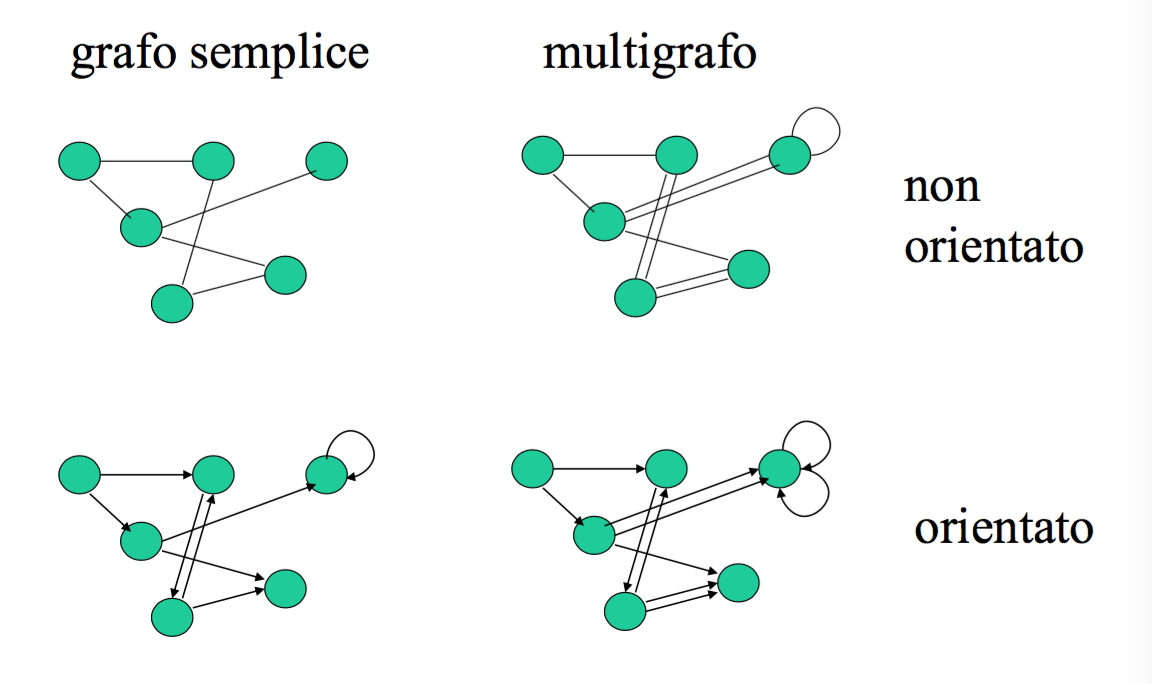
\includegraphics[width=0.75\textwidth]{./notes/immagini/l2-grafi.png}
\caption{Varie tipologie di grafi}
\end{figure}

Se un grafo è semplice, un arco può essere espresso con:

$$
e = uv \in E \text{, con } u,v \in V
$$

e si dice che l'arco \emph{e} è incidente in \emph{u} e \emph{v}. Da
notare che se il grafo è orientato
$e = uv \neq vu$ e la terminologia diventa
``l'arco \emph{e} esce da \emph{u} e entra in \emph{v}''.

Il \textbf{grado} di un vertice \emph{v} viene indicato con $\delta(v)$ e rappresenta il numero di archi incidenti in quel
vertice. Se il grafo è ordinato, il suo \textbf{grado uscente} $\delta^+(v)$ è il numero di archi uscenti e il suo \textbf{grado entrante} è $\delta^-(v)$.

Se due vertici sono collegati da un arco, questi vengono detti
\textbf{adiacenti}.

Un \textbf{cammino} di lunghezza \emph{k} da un vertice \emph{u} ad un
vertice \emph{v} in un grafo \emph{G=(V,E)}, è una sequenza di
\emph{k+1} vertici $x_0 \ldots x_k$, tali che 

$$x_0 = u$, $x_k = v$ e $x_{i-1}x_i \in E \forall i = 1\ldots k$$.

Se il cammino ha lunghezza 0, questo viene detto \textbf{nullo}, mentre
se il vertice di partenza coincide con quello di arrivo, il cammino
prende il nome di \textbf{chiuso}.

Un cammino viene detto \textbf{semplice} quanto tutti i vertici che lo
compongono sono distinti, ad eccezione del primo, che può coincidere
con l'ultimo. Un cammino semplice e il primo vertice coincide con
l'ultimo, questo prende il nome di \textbf{ciclo}. L'esempio più
semplice di ciclo è dato da un cappio.

Un grafo \textbf{aciclico} è un grafo che non contiene cicli.

Quando esiste almeno un cammino dal vertice \emph{u} al vertice
\emph{v}, si dice che \emph{v} è \textbf{accessibile} (o
\textbf{raggiungibile}) da \emph{u}. Questa definizione è simmetrica
solamente nel caso di un grafo non orientato.

Un grafo non orientato si dice \textbf{connesso} se esiste almeno un
cammino tra ogni coppia di vertici.

Le \textbf{componenti connesse} di un grafo sono le classi di
equivalenza dei suoi vertici rispetto alla relazione di accessibilità,
ovvero un sottoinsieme di vertici che sono tutti tra loro accessibili.

Nel caso di un grafo orientato, si dice che è \textbf{fortemente
connesso} se esiste almeno un cammino tra ogni vertice del grafo. In
modo analogo è possibile definire le \textbf{componenti fortemente
connesse}

Sia la \textbf{connessione} che la \textbf{connessione forte} hanno le
proprietà:

\begin{itemize}
\item
  \textbf{riflessiva}: se c'è una connessione tra \emph{u} e \emph{v},
  c'è anche tra \emph{v} e \emph{u}
\item
  \textbf{transitiva}: se c'è una connessione tra \emph{u} e \emph{v} e
  tra \emph{v} e \emph{z}, allora c'è anche tra \emph{u} e \emph{z}.
\end{itemize}

Un sotto-grafo del grafo \emph{G=(V,E)} è un grafo \emph{G' = (V', E')}
tale che:

$$
V' \subseteq V \: \text{e} \: E' \subseteq \{ uv : uv \in E \text{ e } u,v \in V' \}
$$

ovvero un grafo che ha alcuni vertici e alcuni archi del grafo iniziale.
Da notare che se tolgo un vertice, devo togliere anche tutti gli archi
incidenti in quel vertice.

Se il sotto-grafo viene ottenuto rimuovendo solo dei vertici, questo
prende il nome di \textbf{indotto}, perché la rimozione degli archi
viene forzata dalla rimozione dei vertici.

\subsection{Rappresentazione dei
grafi}\label{rappresentazione-dei-grafi}

Per rappresentare i grafi in un calcolatore è possibile utilizzare la
matrice delle adiacenze o la lista delle adiacenze.

\begin{figure}[htbp]
\centering
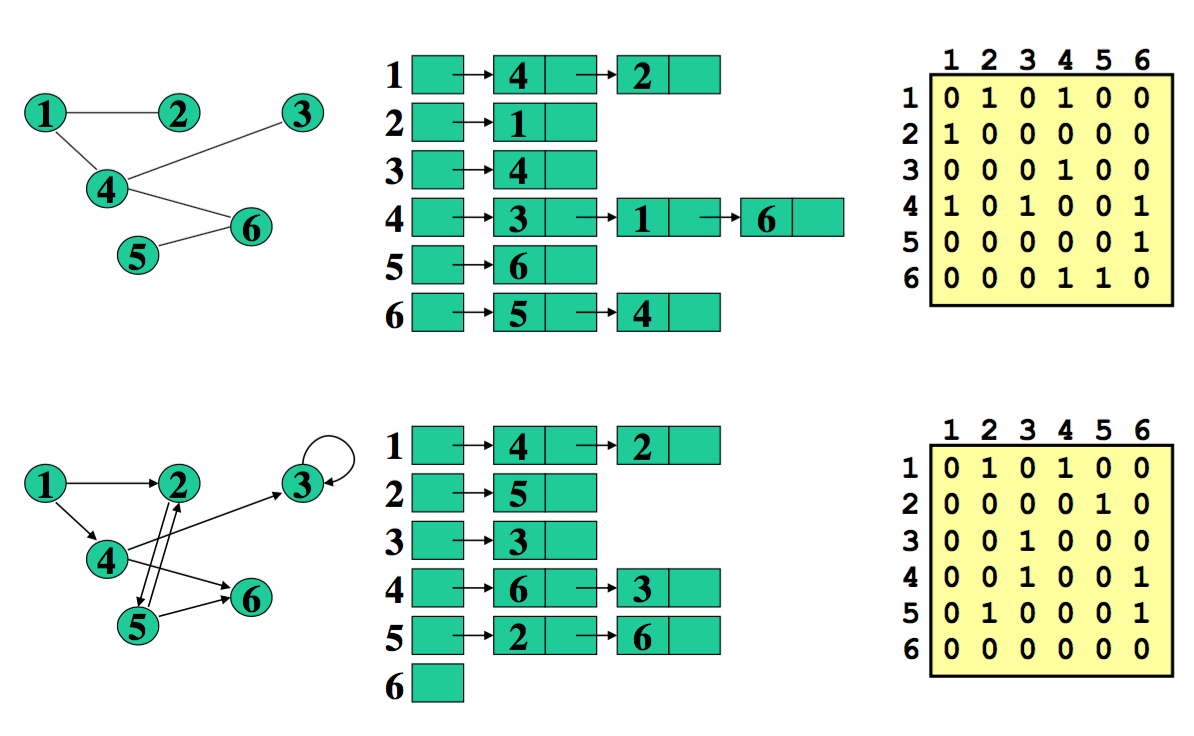
\includegraphics[width=0.75\textwidth]{./notes/immagini/l2-rappr.png}
\caption{Rappresentazione dei grafi}
\end{figure}

\subsubsection{~Lista delle adiacenze}\label{lista-delle-adiacenze}

Per ogni vertice del grafo viene tenuta in memoria una lista \textit{Adj} dei vertici
adiacenti al vertice:

$$
Adj[u] = \{v | uv \in E\} \: \forall u \in V 
$$

Questa rappresentazione richiede memoria per:

\begin{itemize}
\tightlist
\item
  \textit{n\ =\ \textbar{}V\textbar{}} puntatori alla cima delle liste
\item
  \textit{m\ =\ \textbar{}E\textbar{}} elementi per le liste (in totale)
  se il grafo orientato, se è non orientato è \textit{2m}.
\end{itemize}

\subsubsection{Matrice delle adiacenze}\label{matrice-delle-adiacenze}

Viene utilizzata una matrice booleana quadrata che tante righe e tante
colonne, quanti sono i vertici del grafo.

Ogni elemento della matrice vale 1 se i due vertici sono adiacenti, 0
altrimenti:

$$
a_{u,v} = 1 \text{ se } uv \in E
$$

Se il grafo è non orientato, la matrice delle adiacenze è simmetrica.

Il consumo di memoria è $n^2$.

Se il grafo è \textbf{sparso}, ovvero il grado dei vertici è minore del
logaritmo del numero dei vertici, la matrice delle adiacenze risulta
peggiore della rappresentazione con liste in termini di memoria
occupata.

Più formalmente, assumendo che il grafo abbia \textit{n} vertici e \textit{m} archi e che, sia i puntatori, sia gli interi, occupino 32 bit.

Si ha che la lista delle adiacenze occupa $32(n+2m)$, mentre la matrice richiede $n^2$.

La matrice risulta quindi vantaggiosa quando:

\begin{align*}
	32(n+2m) &< n^2 \\
	m &< \frac{n(n-32)}{64}
\end{align*}


\subsection{Calcolo del grafo trasposto}\label{calcolo-del-grafo-trasposto}

Dato un grafo orientato \emph{G=(V,E)} si vuole ottenere $ G^T = (V, E^T)$ in modo che gli archi siano rovesciati, ovvero $E^T = \{uv | vu \in E\}$.

Utilizzando la rappresentazione con la matrice delle adiacenze, è
necessario attraversare metà della matrice e mettere a 1 la cella
\emph{i,j} se \emph{j,i} è a 1. La complessità risulta quindi essere
$O(n^2)$.

Con la lista delle adiacenze l'algoritmo risulta essere


\begin{algorithm}
	\begin{algorithmic}[1]
		\Function{Trasponi}{$Adj,\: Adj^T,\: n$}
			\For{$v = 1 \: to \: n$}
				\State $Adj^T[v] \gets nil$
			\EndFor
			\For{$u = 1 \: to \: n$}
				\State {$x \gets Adj[u]$}
				\While{$x \neq nil$}
					\State{$v \gets x.v$}
					\State{$y \gets nodo(u, Adj^T[v])$}
					\State{$Adj^T[v] \gets y$}
				\EndWhile
			\EndFor
		\EndFunction
	\end{algorithmic}
	\caption{Trasponi: calcolo del grafo trasposto utilizzando la rappresentazione con la lista delle adiacenze}
\end{algorithm}

Ovvero viene attraversata la lista delle adiacenze del grafo originale,
e per ogni elemento delle liste, lo aggiunge ``\emph{al contrario}''
nella nuova lista delle adiacenze.

La complessità risulta quindi essere \emph{O(m+n)}, questo perché il
secondo \texttt{for} esamina tutti i possibili archi, quindi anziché
avere complessità \emph{n} (numero di vertici) ha complessità \emph{m}
(numero di archi).

\subsection{(Esercizio) Ricerca del pozzo
universale}\label{esericizio-ricerca-del-pozzo-universale}

Un vertice è un \textbf{pozzo universale} se può essere raggiunto da
tutti gli altri vertici del grafo, dal quale però non è possibile
raggiungere altri vertici.

Trovare un algoritmo che riesce a risolvere il problema in \emph{O(n)}.


\begin{verbatim}
	- Si cerca un arco tra il nodo 2 -> 1
		- se il bit è a 1, 2 non è un pozzo universale
		- si passa al successivo fino a che non si trova uno nodo che va verso 1,  ad esempio 4->1 a 0
			- in questo modo è possibile escludere il nodo 1
		- in questo modo posso partire dal k+1 in questo caso 5
			- 6->5
				se 0, escludo il 5
				se 1, escludo il 6
		- questo si ripete fino a che non rimane almeno un candidato pozzo
		- Se non c'è nessun canditato, non può esserci un pozzo
		- Se c'è un candidato è necessario verificare che sia un pozzo (forse)
		  la complessità è quindi O(n+n)
\end{verbatim}
	% !TEX encoding = UTF-8
% !TEX program = pdflatex
% !TEX root = InformationRetrieval.tex
% !TEX spellcheck = it-IT

% 6 Ottobre 2016

%\chapter{Rappresentazione dei documenti}
%\section{Analisi automatica del testo}

Tutto è iniziato quando George K. \textbf{Zipf}, uno studioso americano di linguistica ha formulato delle leggi empiriche che mettono in relazione la \textbf{frequenza di una parola} con la sua \textbf{forma} e \textbf{significato}. 
Solo in un secondo momento queste leggi sono state applicate all'indicizzazione dei documenti.

L'osservazione di partenza è stata quella che ci sono poche parole che sono veramente molto frequenti, come gli articoli, e che sono poco significative rispetto il contenuto informativo del documento. Ci sono poi tante parole poco frequenti, alcune delle quali sono fortemente correlate al contenuto informativo del documento. Il gioco è quindi quello di sfruttare al meglio tali parole.

Questo andamento può essere rappresentato graficamente, prima andando a contare le frequenze delle singole parole, per poi andare ad ordinarle da quella più frequente a quella meno frequente. La distribuzione così ottenuta è intera, ma può essere approssimata da un'iperbole.

Tipicamente in inglese:
\begin{itemize}
	\item Le due parole più frequenti sono \textit{the} e \textit{of}, mediamente sono il 10\% delle parole del documento.
	\item Le 6 parole più frequenti corrispondo a circa il 20\% delle occorrente e le 50 parole più frequenti corrispondo a circa il 40\% dei testi. Questo deriva dal fatto che la lingua deve essere ridondante in modo che sia facile da capire.
	\item Considerando un'insieme di documenti molto ampio, circa la metà delle singole parole di quel campione compare una sola volta. Queste sono parole più significative dal punto di vista dell'informazione. Tuttavia è necessario tenere conto che in questo insieme di parole possono comparire anche gli errori di battitura.
\end{itemize}

\subsection{Legge di Zipf}

La legge di Zipf afferma che dato un campione di testi e calcolata la frequenza $f$ delle parole, una volta che si sono messe le parole in ordine decrescente di frequenza, cioè si sono ordinate le parole in base al ragno \textit{r}, la distribuzione che si ottiene ha un andamento assimilabile ad una iperbole e si ha che

$$
r \times f = k
$$

ovvero la distribuzione è data da $ f = \cfrac{k}{r}$.

Se anziché ragionare in termini di frequenza assoluta si passa a considerare quella relativa, ovvero la probabilità osservata di occorrenza della parola, la legge di Zipf può essere riscritta come 

$$
r \times P_r = c
$$

Dove $P_r$ è la probabilità di occorrenza della parola che occupa il rango $r$-esimo e $c$ è una costante ($c = 0.1$ per l'inglese).

Si ha che per la lingua inglese $c \approx 0,1$ e l'iperbole che si ottiene è riportata in figura \ref{fig:zipf}

\begin{figure}[htbp]
\centering
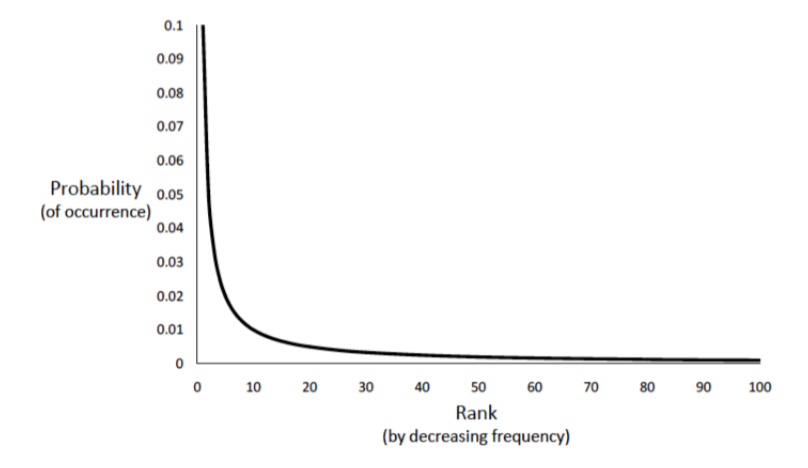
\includegraphics[width=0.55\linewidth]{images/l3-zipf}
\caption{Rango rispetto la probabilità di occorrenza assumendo valida la legge di Zipf con $c = 0.1$}\label{fig:zipf}
\end{figure}

\subsection{Indicazioni di H.P. Luhn}

L'idea per l'indicizzazione è quindi quella di definire due soglie di \textit{cut-off} per evitare di prendere in considerazione le parole troppo frequenti, perché poco significative, e quelle troppo poco, per limitare l'effetto degli errori di battitura.

Ogni parola ha un certo \textbf{resolving power}, ovvero una certa capacità di discriminare il contenuto del documento da quello degli altri e di caratterizzare il contenuto della collezione.

\begin{figure}[htbp]
	\centering
	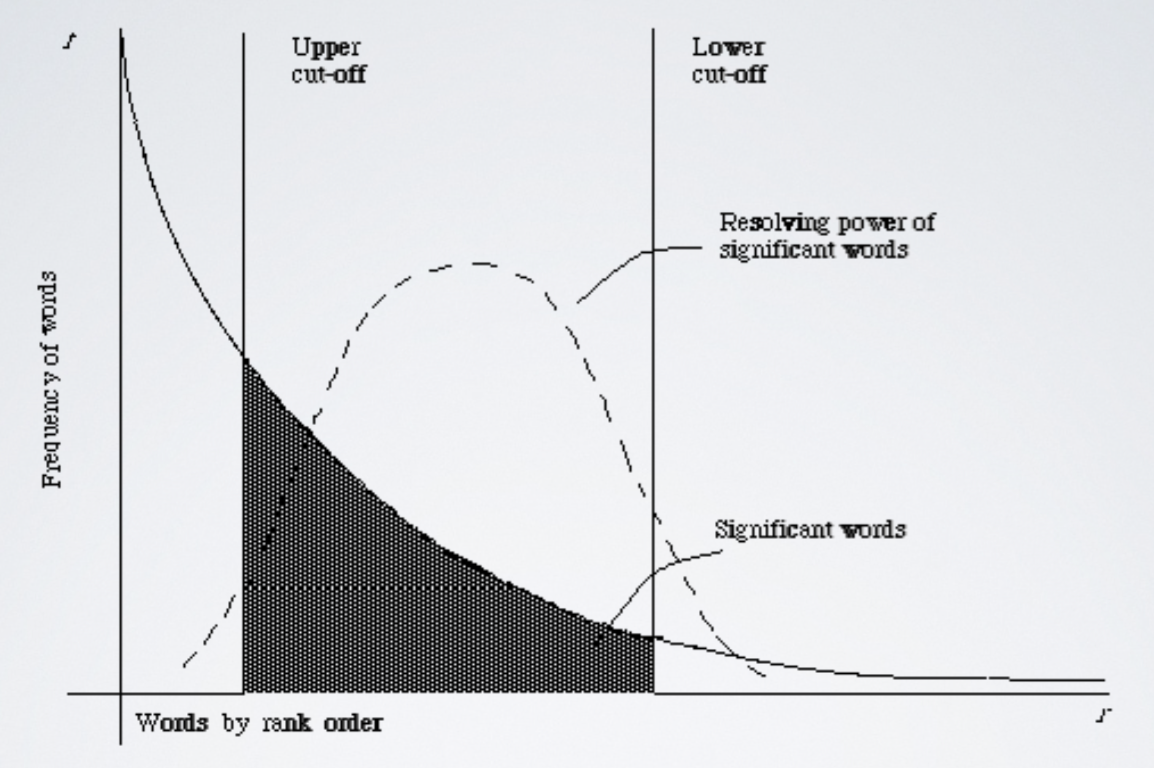
\includegraphics[width=0.55\linewidth]{images/l3-cutoff}
	\caption{Plot della curva $r \times f$ che evidenzia la posizione delle parole significative.}
\end{figure}

Questo vale per le collezioni generiche dei documenti, mentre se si parla di un argomento specifico si può dare maggiore peso a determinate parole. Ad esempio può capitare in che se viene preso in esame un manuale di MySQL è ovvio che le parole ``MySQL'' e  ``table'' compariranno tante volte anche se non sono articoli.

C'è anche un altro discorso relativo alla forma plurale, che in conteggio di frequenza vengono considerate come diverse, quando in realtà può essere che abbia lo stesso valore informativo della forma singolare. In alcuni casi è quindi opportuno sommare le occorrenze della forma plurale e di quella singolare.

Si ha quindi che i passi per applicare le indicazioni di Luhn sono:

\begin{itemize}
	\item Si calcoli la frequenza di ogni descrittore in ogni documento della collezione di riferimento. C'è inoltre da scegliere come trattare le parti di contorno dei documenti come l'indice, la premessa, ecc. tali parti tipicamente non vengono considerate.
	\item Si calcoli la frequenza totale di ogni descrittore.
	\item Si ordino i descrittori per frequenza decrescente.
	\item Si scelga una soglia di \textit{upper cut-off} e si rimuovano dalla lista i descrittori con frequenza superiore alla soglia. In questo modo si rimuovono gli articoli, le preposizioni, ecc.
	\item Si scelga un'altra soglia di \textit{lower cut-off} e si rimuovano dalla lista i descrittori con frequenza inferiore al valore di soglia. In questo modo si rimuovono i descrittori ``rumore''  o che non apportano alcun contribuito alla descrizione del contenuto.
\end{itemize}

\noindent Entrambe le soglie possono essere calcolate in modo euristico.

Le parole che vengo eliminate dalle soglie di cut-off vengono nominate \textbf{stop word} e sono raccolte nella lista che prende il nome di \textbf{stop list}.


\textbf{{\color{Red} Possibile esercizio:}} Domande relative alle osservazioni proposte da Zipf e Luhn.

\section{Indicizzazione}

L'indicizzazione ha l'obiettivo di rappresentare il contenuto informativo di un documento e nel tempo questo processo ha preso una struttura a fasi.

Il documento viene rappresentato da dei descrittori che vengono utilizzati per la costruzione degli indici, utili al reperimento dell'informazione.

Quindi l'indicizzazione fornisce automaticamente una rappresentazione più compatta e direttamente utilizzabile del contenuto informativo del documento. Gli indici sono utilizzati come surrogati del contenuto del documento durante la fase di reperimento.

L'indicizzazione può essere svolta:
\begin{itemize}
	\item manualmente
	\item in modo automatico
	\item in modo semi-automatico, quando è necessario intervenire all'interno del processo per prendere delle decisioni che non possono essere prese in modo automatico.
\end{itemize}

\noindent Tutti questi metodi funzionano estraendo direttamente dal documento le informazioni. Tuttavia possono essere estesi in modo che vengano presi in considerazione anche dei dizionari o delle meta-informazioni.

\begin{figure}[htbp]
	\centering
	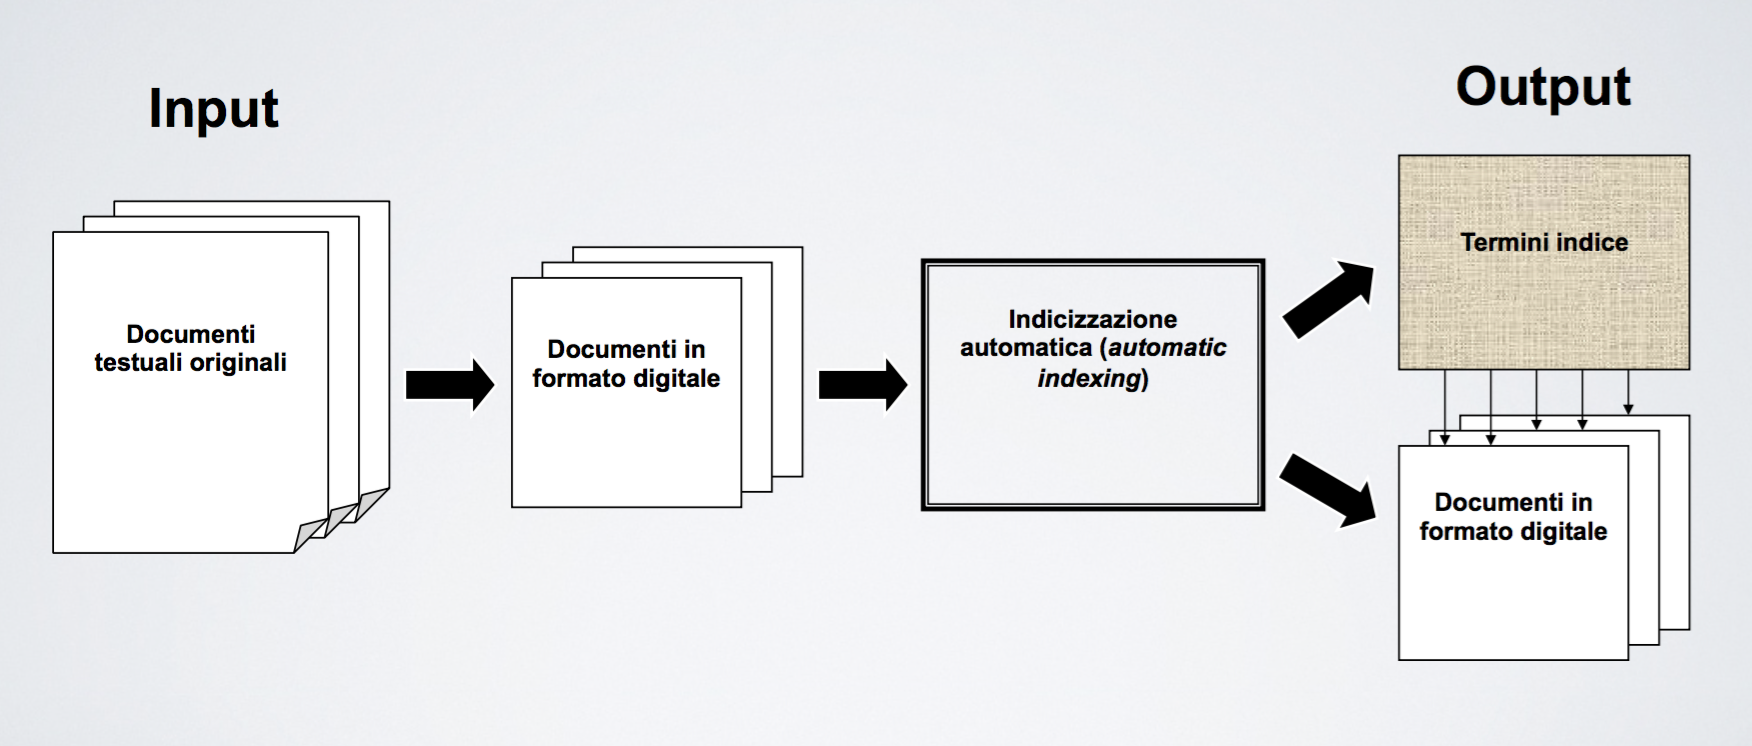
\includegraphics[width=0.7\linewidth]{images/l3-indicizzazione}
	\caption{Schema generale dell'indicizzazione}
\end{figure}

\subsection{Indicizzazione automatica dei testi}

L'indicizzazione automatica di un documento testuale è un processo che esamina automaticamente gli oggetti informativi (parole, frasi, didascalie, figure, ecc.) che compongono il documento e produce una lista di termini indice presenti nell'intera collezione dei documenti.

L'estrazione dei termini indice viene fatta da appositi algoritmi e, una volta estratti, questi vengono collegati ai diversi documenti che li contengono.
Così facendo durante il reperimento sarà sufficiente fare riferimento ai termini indice e non all'intera collezione.

\subsection{Attuazione dell'indicizzazione automatica}

L'indicizzazione automatica dei documenti testuali viene eseguita in più fasi, che devono essere attuate in sequenza:

\begin{enumerate}
	\item Analisi lessicale e selezione delle parole.
	\item Eventuale rimozione delle stop word.
	\item Riduzione delle parole originali alle rispettive radici (\textit{STEM}). Ad esempio le forme plurali vengono ridotte a quelle singolari.
	\item Composizione dei termini. Come ad esempio ``information retrieval''. Ovvero le parole vengono combinate tra loro quando si trovano ad una determinata distanza.
	\item Creazione dell'indice.
	\item Eventuale pesatura degli elementi dell'indice. 
\end{enumerate}

Alla fine di queste fasi l'indice sarà composto da parole, termini e frasi che noi riteniamo significative, assieme alle informazioni del peso che gli diamo e alla loro frequenza all'interno dei documenti.








	
	% !TEX encoding = UTF-8
% !TEX program = pdflatex
% !TEX root = MEMOC.tex
% !TEX spellcheck = it-IT

% 20 Ottobre 2016
% Section Modellazione di un problema
% Subsection Lettura dei giornali
% Subsubsection Modellazione

% esercizio delle costruzione della barca.
\subsection{Costruzione di una barca (Esercizio 3)}

La costruzione di una barca da diporto comporta il completamento delle operazioni indicate nella tabella che segue, che ne riporta anche la durata in giorni.

\begin{table}[htbp]
	\centering
	\begin{tabular}{ccc}
		\textbf{Operazione} & \textbf{Durata} & \textbf{Precedenze} \\ \hline
		A                   & 2               & nessuna             \\ 
		B                   & 4               & A                   \\ 
		C                   & 2               & A                   \\ 
		D                   & 5               & A                   \\ 
		E                   & 3               & B,C                 \\ 
		F                   & 3               & E                   \\ 
		G                   & 2               & E                   \\ 
		H                   & 7               & D,E,G               \\ 
		I                   & 4               & F,G                 \\ 
	\end{tabular}
\end{table}

Si consideri che alcune operazioni sono in alternativa. In particolare, bisogna eseguire solo una tra le operazioni B e C, e solo una tra le operazioni F e G. Inoltre, se si eseguono sia C che G, la durata dell'operazione I si allunga di 2 giorni.
La tabella indica anche, per ogni operazione, l'insieme delle precedenze (operazioni che devono essere completate prima di poter eseguire l'operazione stessa).
Scrivere un modello di programmazione lineare per decidere quali operazioni in alternativa eseguire, con l'obiettivo di minimizzare la durata complessiva delle operazioni di costruzione.

\subsubsection{Modellazione}

Le scelte in questo caso riguardano quali attività svolgere, tra quelle che possono essere eseguite in alternativa al fine di minimizzare il makespan.

Dal momento che si vuole minimizzare la durata, conviene scegliere dopo quanti giorni dall'inizio dei lavori deve terminare una determinata attività:

$$
t_i \quad \text{dopo quanti giorni termina l'attività }i \in A = \{A, \ldots, I \}
$$

\noindent Così risulta facile definire la funzione obiettivo

$$
\min z
$$

\noindent dove \textit{z} è il makespan, ovvero il giorno in cui termina l'ultima attività da eseguire. Per specificare ciò nel modello serve il vincolo

$$
z \geq t_I
$$

\noindent \`E necessario poi modellare le varie precedenze tra le attività e il fatto che non due attività non possono essere eseguite in parallelo.
Questo viene fatto con una serie di vincoli del tipo:

$$
t_i \geq t_{j} + d_{i} \forall \: i \in A, j \in prec(i)
$$

\noindent dove $d_i$ è la durata dell'attività $i$ e $prec(i)$ è l'insieme delle attività che devono essere svolte prima di $i$. Ad esempio: $prec(H) = \{D,E,G\}$.

Resta poi da modellare il fatto che alcune attività possono essere svolte in alternativa. In questo servono delle variabili binarie $y_i$, una per ogni attività che può essere eseguita e che indicano l'attività viene svolta o meno.

Per vincolare la scelta tra due attività è necessario aggiungere i vincoli del tipo

$$
y_i + y_j = 1
$$

\noindent dove $i$ e $j$ sono due attività che possono essere eseguite in alternativa.

\`E inoltre necessario modificare alcuni dei vincoli riguardo le precedenze, perché se un'attività non viene svolta, questa non deve essere presa in considerazione nella pianificazione:

$$
t_i \geq t_{j} + d_i - M(1 - y_i)
$$ 

\noindent Così facendo, se la soluzione prevede che l'attività $i$ non venga svolta ($y_i = 0$), il vincolo diventa ridondante e non va ad influenzare il makespan.
Con i dati del problema alcuni di questi vincoli sono:

\begin{align*}
	t_B &\geq t_{A} + d_B - M(1 - y_B) \\
	t_C &\geq t_{A} + d_C - M(1 - y_C)
\end{align*}

C'è inoltre da modellare il fatto che se vengono eseguite determinate attività la durata di altre attività aumenta.

Serve quindi una variabile booleana $c$ che specifica se questa condizione si verifica. Questa variabile viene poi utilizzata per aggiornare i vincoli relativi alle attività interessate. Ad esempio per i dati del problema si ha

\begin{align*}
	&y_C + y_G \leq 1 + c \quad \text{attivazione di \textit{c}} \\
	&t_I \geq t_F + d_I + 2c \quad \text{aumento della durata per l'attività \textit{I} se vale \textit{c}} \\ 
	&t_I \geq t_G + d_I + 2c \quad \text{''} \\
\end{align*}

\noindent Rimane infine da specificare i domini delle variabili:

\begin{align*}
	t_i &\in \mathbb{R} \: \forall \: i \in A \\
	y_i, c, &\in \{0,1\} \\
	z &\in \mathbb{R}
\end{align*}

\noindent Servono poi i parametri $d_i \in \mathbb{R}$ che rappresentano le durate e la costante $M$ che rappresenta un numero sufficientemente grande in grado di rendere ridondanti i vincoli in cui compare.

\subsection{Turni delle farmacie (Esercizio 5)}

La federazione dei farmacisti vuole organizzare i turni festivi delle farmacie sul territorio regionale. 
\`E stabilito a priori il numero dei turni, che devono essere bilanciati in termini di numero di farmacie, considerando che ciascuna farmacia deve appartenere, per equità, a un solo turno. 
Ad esempio, se il numero complessivo di farmacie è 12 e si vogliono organizzare tre turni, ciascun turno sarà formato da quattro farmacie. 
Sia le farmacie che gli utenti si considerano distribuiti sul territorio e concentrati in centroidi (corrispondenti in genere con comuni o quartieri). 
Per ogni centroide sono noti il numero di utenti e il numero di farmacie. \`E inoltre nota la distanza tra ogni coppia ordinata di centroidi. 
In prima istanza, si trascurano problemi relativi alla congestione e si assume che gli utenti, in ciascun turno, si servano dalla farmacia aperta più vicina. 
Si vuole determinare la distribuzione dei turni festivi che minimizza la distanza complessiva percorsa dagli utenti per il servizio festivo.

\subsubsection{Modellazione}

In questo caso vogliamo decidere quale farmacia fa quale turno, in modo che ci sia una buona copertura del territorio, assumendo che le persone vadano nella farmacia più vicina.

L'obiettivo è quindi quello di minimizzare la strada che devono fare le persone per raggiungere le farmacie di turno.

Di sicuro serve una variabile che specifica quale farmacia è aperta in quale turno.

$$
y_{i,k} = \begin{cases}
1 \quad &\text{la farmacia \textit{i} è aperta nel turno \textit{k}} \\
0 \quad &\text{altrimenti}
\end{cases}
$$

\noindent con $i \in P$ e $k \in 1 \ldots K$. Dove $P$ è l'insieme delle farmacie e $K$ è il numero di turni che si voglio fare.

Per esprimere la nostra funzione obiettivo servono altre variabili, perché dobbiamo anche prendere in considerazione la distanza delle farmacie, in modo da poterla minimizzare.

Ci sarà quindi il set $C$ di clienti che devono essere serviti e dei parametri che specificano la distanza $D_{j,i}$ che c'è tra un cliente $j \in C$ e la farmacia $i \in P$.
Tuttavia la distanza che l'utente deve fare \textbf{dipende dalle farmacie aperte} in un determinato turno e quindi non conviene utilizzare direttamente il parametro, in quanto in base al turno la distanza è variabile.

Conviene quindi aggiungere una variabile che specifica quanta strada il cliente $j$ deve fare durante il turno $k$ per raggiungere la farmacia più vicina aperta.

$$
d_{j,k} \: \text{distanza tra il cliente \textit{j} e la farmacia più vicina durante il turno \textit{k}}
$$

\noindent Bisogna però in qualche modo collegare le variabili $d_{j,k}$ con l'apertura/chiusura delle farmacie.

Serve quindi un modo per discriminare in quale farmacia va l'utente in un determinato turno:

$$
x_{j,i,k} = \begin{cases}
1 \quad & \text{se \textit{j} va nella farmacia \textit{i} durante il turno \textit{k}} \\
0 \quad &\text{altrimenti}
\end{cases}
$$

\noindent Così facendo risulta semplice trovare un valore per i $d_{j,k}$, perché basta il vincolo:

$$
d_{j,k} = \sum\limits_{i \in P} D_{j,i} x_{j,i,k} \quad \forall \:j \in C, k \in K
$$

\noindent Con questo vincolo viene presa in considerazione solo una distanza per ogni turno, perché durante un turno il cliente va sempre nella farmacia più vicina e quindi, fissati un $j$ e un $k$, ci sarà solo un $x_{j,i,k}$ che vale 1.
Quest'ultima cosa il risolutore non lo sa e quindi bisogna aggiungere gli opportuni vincoli:

$$
\sum\limits_{i \in P} x_{j,i,k} = 1 \quad \forall \: j \in C, k \in K
$$

\noindent Manca ancora il vincolo che ogni farmacia faccia esattamente un turno, il quale può essere semplicemente aggiunto con una sommatoria sulle $y_{i,k}$:

$$
\sum\limits_{k = 1}^{K} y_{i,k} = 1 \quad \forall \: i \in P
$$

\noindent Per completare il modello rimane da collegare le $x$ con le $y$, perché ovviamente un cliente non può andare in una farmacia chiusa.

$$
x_{j,i,k} \leq y_{j,k} \quad \forall \: i,j,k
$$

\noindent La funzione obiettivo risulta quindi essere:

$$
\min \sum\limits_{j \in C}\sum\limits_{k = 1}^{K} d_{j,k}
$$

\noindent Rimane inoltre da imporre che ogni turno sia bilanciato, ovvero che ci sia sempre un numero simile di farmacie aperte:

$$
\bigg\lfloor \frac{|P|}{K} \bigg\rfloor \leq \sum\limits_{i \in P} y_{i,k} \leq  \bigg\lceil \frac{|P|}{K} \bigg\rceil \quad \forall \: k
$$

\noindent Rimane da specificare i domini delle variabili:

\begin{align*}
	y_{i,k} &\in \{0,1\} \\
	x_{j,i,k} &\in \{0,1\} \\
	d_{j,k} &\in \mathbb{R}
\end{align*}

\noindent Peccato che ci sia un problema. Con i vincoli attuali abbiamo espresso che per ogni turno un cliente va sempre nella stessa farmacia e che quella farmacia deve essere aperta, ma non viene specificato che il cliente va alla farmacia più vicina.

In realtà questo non è un problema, perché è durante il processo di ottimizzazione che viene impostata che le varie distanze vengono minimizzate.

Questo perché \textbf{l'obiettivo di un modello è quello di descrivere le caratteristiche di una soluzione}, mentre è il risolutore che cercando la soluzione ottima effettua la minimizzazione. Infatti, una soluzione che manda un cliente in una farmacia diversa da quella aperta che gli è più vicina, è comunque una soluzione accettabile, ma di sicuro non è ottima e quindi viene scartata.

\paragraph{Osservazione - Simmetrie}

Una volta trovata una soluzione ottima per questo problema si può osservare che permutando l'ordine dei turni ottenuto si ottiene un'altra soluzione ottima con un ordine diverso.

Questo è causato dal fatto che una volta scelte le farmacie che sono aperte nei vari turni, l'ordine in cui sono effettuati i turni è indifferente, ottenendo così una soluzione simmetrica. 
La presenza di queste simmetrie è tipicamente un problema perché può portare ad un'esplosione combinatoria delle soluzioni.

L'origine di queste simmetrie è tipicamente causata dal modello, in questo caso il problema deriva dal fatto che viene dato ``\textit{un nome}'' ai turni e non sempre è possibile ri-modellare il problema in modo che non ci siano simmetrie.

\subsubsection{Modellazione alternativa}

Dato che abbiamo un'insieme di farmacie $P$ e che ogni farmacia fa solo un turno, possiamo vedere un turno come un sottoinsieme di $P$.

La scelta dei turni diventa quindi una scelta di quali sottoinsiemi selezionare dall'insieme delle parti $2^P$.

Questa scelta può essere modellata con una variabile binaria

$$
x_J = \begin{cases}
1 \quad& \text{se il sottoinsieme \textit{J} è un turno} \\
0 \quad&\text{altrimenti}
\end{cases} \quad \forall \: J \subset P, J \in 2^P
$$

\noindent Con questa variabile non ci sono simmetrie in quanto la variabile è direttamente collegata al turno che rappresenta.

La minimizzazione da fare diventa quindi ($j$ rappresenta i clienti, $J$ il turno)

$$
\min \sum\limits_{J \in 2^P} \sum\limits_{j \in C} D_{j,J}x_J
$$

\noindent Nella funzione obiettivo non compare più la variabile $d_{j,k}$, ma compare un parametro $D_{j,J}$, questo perché nella formulazione precedente la composizione dei vari turni era variabile e di conseguenza anche la distanza cambiava in base alla composizione del turno, mentre con questo nuovo modello so a priori quali sono le farmacie che appartengono ad un determinato turno e quindi per ogni turno e per ogni cliente posso pre-calcolare la distanza minima.

Ci sono poi altri vincoli che devono essere ri-formulati.

Per specificare che si siano esattamente $K$ turni, basta effettuare la sommatoria sulle $x_J$.

$$
\sum\limits_{J \in 2^P} x_J = K
$$

\noindent Bisogna inoltre imporre il vincolo che ogni farmacia faccia esattamente un turno, perché al momento la stessa farmacia può comparire in più turni (sottoinsiemi).

In questo caso serve un'ulteriore \textbf{parametro} che specifichi se una farmacia è in un determinato turno.

$$
A_{i,J} = \begin{cases}
1 \quad &\text{se } i \in J \\
0 \quad &\text{altriment}
\end{cases} \quad \forall \: J \in 2^P
$$

\noindent Da notare che è un parametro e non una variabile perché è un valore che può essere pre-calcolato quando viene costruito l'insieme delle parti.

Con questi parametri risulta semplice porre il vincolo che una farmacia faccia al massimo un turno.

$$
\sum\limits_{J \in 2^P} A_{i,J} x_J = 1 \quad \forall \: i \in P
$$

\noindent Rimane da modellare il fatto che i turni devono essere bilanciati, ma per fare questo non servono nuovi vincoli. Infatti basta considerare, al posto di tutto l'insieme delle parti $2^P$, un suo sottoinsieme $G$ composto solamente dai sottoinsiemi di $P$ che hanno cardinalità simile.

$$
G = \bigg\{x \:  | \: x \in 2^P, \bigg\lfloor \frac{|P|}{K} \bigg\rfloor \leq |\:x\:|\leq  \bigg\lceil \frac{|P|}{K} \bigg\rceil \bigg\}
$$

\noindent Questo modello non ha simmetrie ed è molto semplice, tuttavia soffre di un grande problema: se ci sono $100$ farmacie, il calcolo dell'insieme delle parti di $P$ e dei parametri può richiedere troppo tempo a causa della crescita esponenziale della cardinalità dell'insieme delle parti.










	%\appendix
	\part{Laboratorio}
	% !TEX encoding = UTF-8
% !TEX program = pdflatex
% !TEX root = MEMOC.tex
% !TEX spellcheck = it-IT

\chapter{Laboratorio 1}

\section{Introduzione}

Come solver per i nostri modelli utilizzeremo CPLEX.

Un solver è un'applicazione che prende in input la descrizione di un modello relativo ad un problema di ottimizzazione e fornisce in output una soluzione ottima del problema.

\begin{figure}[htbp]
	\centering
	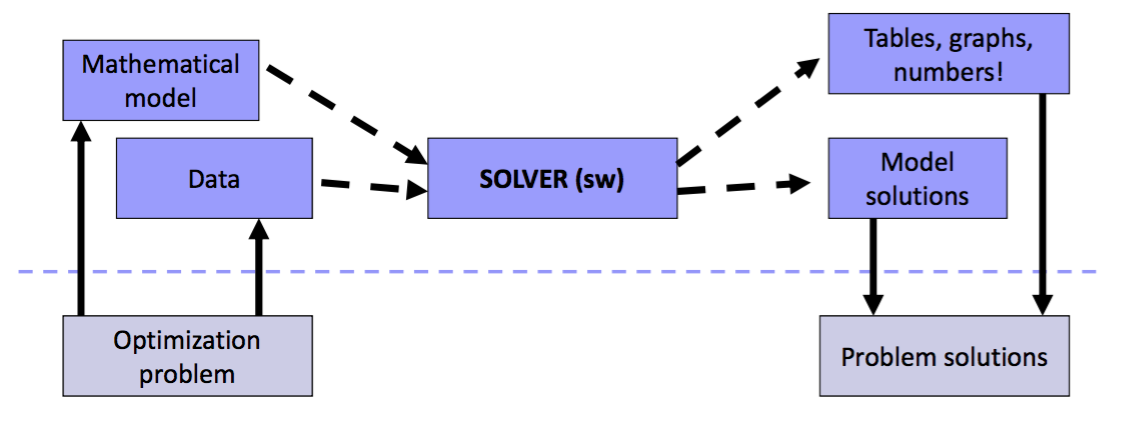
\includegraphics[width=0.7\linewidth]{./images/lab1-schema-1}
\end{figure}

Ovviamente il modello deve essere espresso in una particolare sintassi.

CPLEX è un solver MILP, ovvero un solver in grado di risolvere problemi di programmazione lineare intera mista.
Questa tipologia di solver è quella più comune perché è molto efficiente, non soffre di problemi legati alla stabilità numerica e risulta facilmente embeddabile in altri programmi.

Come anticipato, ogni solver ha una sua interfaccia che può essere utilizzata da dei linguaggi special-purpose o general-purpose.

\begin{figure}[htbp]
	\centering
	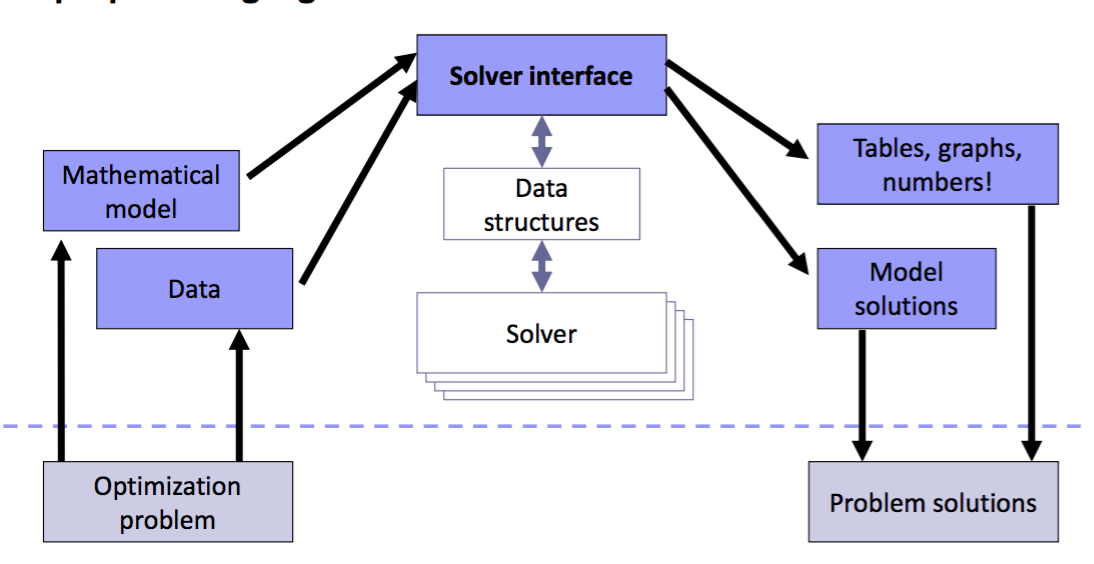
\includegraphics[width=0.7\linewidth]{./images/lab1-schema-2}
\end{figure}

\section{Introduzione a CPLEX}

CPLEX è stato uno dei primi solver e al momento è tra i migliori, in quanto include lo stato dell'arte delle varie tecnologie.

Ci sono varie interfacce utilizzabili per i vari linguaggi di programmazione più diffusi e anche per i linguaggi special-purpose come AMPL. Noi utilizzeremo le API C/C++.

Le \textbf{CPLEX Callable Libraries} implementano varie algoritmi di risoluzione, noi utilizzeremo il MIP, e sono composte da due oggetti principali: \texttt{Environment} e \texttt{Problem}.

\begin{itemize}
	\item \texttt{Enviroment}: contiene le informazioni relative ai parametri di ottimizzazione, alla configurazione, ecc.
	\item \texttt{Problem}: contiene le informazioni di un particolare problema, come i vincoli e le variabili.
\end{itemize}

\noindent\`E necessario che venga definito almeno un \texttt{Environment} e un \texttt{Problem}.

\begin{verbatim}
CPXENVptr CPXopenCPLEX / CPLcloseCPLEX
CPXLPptr CPLcreateprob / CPXfreeprob
\end{verbatim}

\noindent Per interagire con gli oggetti vengono usate le apposite API che seguono più o meno lo stesso schema

\begin{verbatim}
int CPXfuncName (eviroment[,problem],...);
\end{verbatim}

\noindent L'intero ritornato è un codice errore, se è 0 vuol dire che l'operazione è andata a buon fine.

\section{Rappresentazione con matrici sparse}

Un modello generico può essere rappresentato da delle matrici:

\begin{align*}
\min/\max & C^T x \\
\st & A x = b \\
	& x \geq 0
\end{align*}

\noindent con $x,C \in \mathbb{R}^n$, $A \in \mathbb{R}^{m \times n}$ e $b \in \mathbb{R}^m$.

Nei casi reali la matrice $A$ risulta essere molto grande e sparsa, ovvero con molti elementi uguali a 0.

Questa matrice viene quindi rappresentata con 3 vettori:

\begin{itemize}
	\item \texttt{double* val}: contiene i valori della matrice in modo compatto (uno dietro l'altro).
	\item \texttt{int* idx}: contiene l'indice della colonna del valore che si trova alla stessa posizione del vettore \texttt{val}. La lunghezza di \texttt{idx} è la stessa di \texttt{val}.
	\item \texttt{int* beg}: contiene gli indici per il vettore \texttt{val} dove iniziano le righe della matrice.
\end{itemize}

\begin{figure}[htbp]
	\centering
	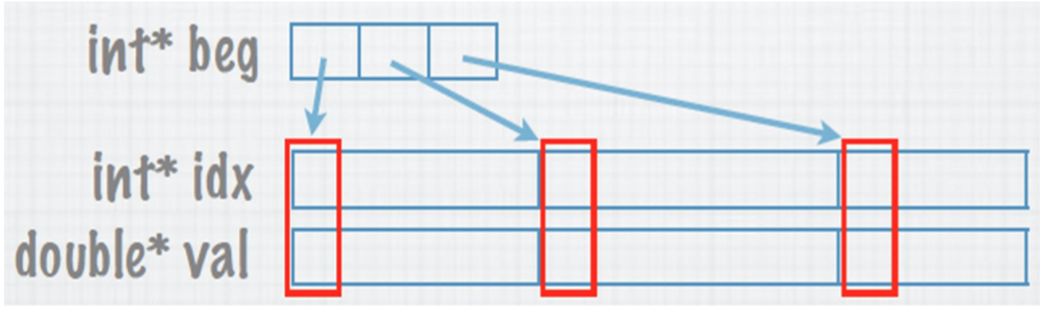
\includegraphics[width=0.5\linewidth]{./images/lab1-matrix}
\end{figure}

\section{Utilizzo di CPLEX}

Per avviare l'ambienti di CPLEX nel terminale è necessario eseguire i comandi:

\begin{verbatim}
$ . clpex_env
$ cplex
\end{verbatim}

\noindent Nel file \texttt{02.firstModel/cpxmacro.h} ci sono delle macro che facilitano la creazione dell'ambiente e del problema.
Abbiamo pure un makefile che compila tutto, che bello!
	
	
	
	
	%%\renewcommand{\glossaryname}{Glossario}

%\newglossaryentry{Cordova}
%{
%	name=\glslink{Cordova}{Cordova},
%	text=Cordova,
%	sort=Cordova,
%	description={Apache Cordova è un framework open source per la realizzazione di applicazioni ibride che offre delle API che permettono di accedere via JavaScript ad alcune funzionalità native del dispositivo, come l'accelerometro o la fotocamera}
%}
\subsection*{A}

\underline{\textbf{ARPA}}: %TODO

\underline{\textbf{ARPANET}}: %TODO

\underline{\textbf{Assembler}}: %TODO

\subsection*{B}

\underline{\textbf{Beowulf}}: %TODO

\subsection*{C}

\subsection*{D}

\underline{\textbf{Debian}}: %TODO

\underline{\textbf{DFSG}}: %TODO

\subsection*{E}

\subsection*{F}

\underline{\textbf{Free Software Foundation}}: %TODO

\underline{\textbf{Freeware}}: %TODO

\underline{\textbf{fsf}}: %TODO

\subsection*{G}

\underline{\textbf{GNU}}: %TODO

\underline{\textbf{GPL}}: %TODO

\subsection*{H}

\subsection*{I}

\subsection*{J}

\subsection*{K}

\underline{\textbf{Kernel}}: %TODO

\subsection*{L}

\underline{\textbf{Linux}}: %TODO

\subsection*{M}

\underline{\textbf{Mimix}}: %TODO

\underline{\textbf{MUTIX}}: %TODO

\subsection*{N}

\underline{\textbf{Netscape}}: %TODO

\underline{\textbf{nslu2}}: %TODO

\subsection*{O}

\underline{\textbf{OSI}}: %TODO

\subsection*{P}

\underline{\textbf{PDP}}: %TODO

\subsection*{Q}

\subsection*{R}

\underline{\textbf{RedHat Enterprise Linux}}: %TODO

\underline{\textbf{Routes}}: %TODO



\subsection*{S}

\underline{\textbf{StarOffice}}: %TODO

\underline{\textbf{Sun}}: 

\underline{\textbf{S\&P}}: %TODO

\underline{\textbf{Shareware}}: %TODO

\underline{\textbf{Symbolics}}: %TODO	

\subsection*{T}

\underline{\textbf{TECO}}: %TODO

\subsection*{U}

\underline{\textbf{Unix}}: %TODO

\subsection*{V}

\subsection*{W}

\subsection*{X}

\subsection*{Y}

\subsection*{Z}


	




	\printindex
	
	
\end{document}